%\nocite{a9a08fe2}
%\nocite{d37d0fca}
%%%
A cobordism between closed manifolds is a manifold with boundary. However, in the following we will have to deal with more general, higher cobordisms between manifolds with boundary which leads to manifolds with corners. Thus we will briefly describe manifolds with corners here and discuss how they serve as such more general codordisms.
\\\\
Manifolds with corners generalize manifolds with boundary in much the same way as manifolds with boundary generalize ordinary manifolds without boundary. Ordinary manifolds locally look like the Euclidean $n$-space $\mathbb{R}^{n}$ for some $n \in \mathbb{N}$ and manifolds with boundary locally look like the Euclidean half-space $\mathbb{R}_{+}^{n} := \mathbb{R}^{n-1} \times [0,\infty)$. As a natural generalization manifolds with corners locally look like $\mathbb{R}_{k+}^{n} := \mathbb{R}^{n-k} \times [0,\infty)^{k}$ for some $0 \leq k \leq n$. More precisely, let $n \geq 1$, let $M$ be a topological\footnote{that is, without a given smooth structure} $n$-manifold with boundary and let $x \in M$. A \textbf{chart with corners (around $x$ of index $k$)}, $k \in \mathbb{N}$, is a homeomorphism $\varphi \colon U \to O$ with $U \subset M$ open and containing $x$ and $O \subset \mathbb{R}_{n+}^{n}$ open, such that $\varphi(x)$ has $k$-many coordinates which take the value zero. Such a chart is often written as a pair $(U,\varphi)$. Now for a map $f \colon S \subset \mathbb{R}_{n+}^{n} \to \mathbb{R}^{m}$, $m \in \mathbb{N}^{\times}$, we say that it is \textbf{smooth} if there is an open subset $\tilde{S} \subset \mathbb{R}^{n}$ containing $S$ and a smooth extension of $f$, that is, a smooth map $\tilde{f} \colon \tilde{S} \to \mathbb{R}^{m}$ with $\tilde{f}\vert S = f$. For $m=n$ we call $f \colon S \to f(S)$ a \textbf{diffeomorphism} if $f$ is bijective and both $f$ and $f^{-1}$ are smooth. Now just as for ordinary manifolds we define that two charts with corners $(U_{1},\varphi_{1})$ and $(U_{2},\varphi_{2})$ are \textbf{compatible} if either $U_{1} \cap U_{2} = \emptyset$ or if the composition
\begin{align*}
  \varphi_{1}
  \circ
  \varphi_{2}^{-1}
  &\colon
  \varphi_{2}(U_{1} \cap U_{2})
  \to
  \varphi_{1}(U_{1} \cap U_{2})
\end{align*}
is a diffeomorphism. As usual such compositions are called \textbf{transition maps}. A set of pairwise compatible charts with corners which covers $M$,
\begin{align*}
  \mathcal{A}
  &=
  \lbrace
    (U_{j},\varphi_{j})
    \colon
    j
    \in
    \mathsf{J}
  \rbrace
  \qquad
  \text{with}
  \qquad
  \bigcup_{j \in \mathsf{J}}
  U_{j}
  =
  M
\end{align*}
is a \textbf{(smooth) atlas (with corners)}. A subset of an atlas with corners that is again such an atlas is a \textbf{subatlas (with corners)}. Two atlases with corners $\mathcal{A}_{1},\mathcal{A}_{2}$ are defined to be \textbf{equivalent} if $\mathcal{A}_{1} \cup \mathcal{A}_{2}$ is an atlas with corners. The union of all atlases in an equivalence class is called a \textbf{maximal atlas (with corners)}. A pair\footnote{we will mostly suppress $\mathcal{D}$ in the notation} $M \doteq (M,\mathcal{D})$ consisting of a topological manifold with boundary $M$ and an equivalence class of atlases with corners $\mathcal{D}$ (or equivalently a maximal atlas) is an \textbf{$n$-(dimensional )manifold with corners} and $\mathcal{D}$ is also called \textbf{corner structure}.
\\
One can show that if two charts around $x \in M$ are compatible, then they are of the same index. Hence, we can define the \textbf{index of $x$}, denoted $\mathrm{index}(x)$, to be the index of any chart around $x$ as this does not depend on the chart. For each $0 \leq k \leq n$ we define the \textbf{index $k$ stratum (of $M$)} to be
\begin{align*}
  \mathcal{S}^{k}(M)
  &:=
  \lbrace
    x \in M
    \colon
    \mathrm{index}(x)
    =
    k
  \rbrace
\end{align*}
Note that $M$ is an ordinary (smooth) manifold precisely if $\mathcal{S}^{k}(M) = \emptyset$ for all $k > 0$ and a (smooth) manifold with boundary precisely if $\mathcal{S}^{k}(M) = \emptyset$ for all $k > 1$. Moreover, it is easy to see that
\begin{align*}
  M
  &=
  \bigsqcup_{k=0}^{n}
  \mathcal{S}^{k}(M)
  \qquad
  \text{and}
  \qquad
  \overline{\mathcal{S}^{k}(M)}
  =
  \bigcup_{j=k}^{n}
  \mathcal{S}^{j}(M)
\end{align*}
where $\bigsqcup$ denotes the disjoint union and $\overline{\mathcal{S}^{k}(M)}$ is the closure of $\mathcal{S}^{k}(M)$ in $M$. The points of $\mathcal{S}^{k}(M)$ can be understood as the corners of codimension $k$ of $M$ so that in particular $\mathcal{S}^{0}(M)$ is the interior $\mathrm{int}(M)$ of $M$ when considered as topological manifold and $\overline{\mathcal{S}^{1}(M)}$ is the boundary $\partial M$ of $M$ when considered as topological manifold.
\\
Many constructions of ordinary manifolds and manifolds with boundary can be carried over to manifolds with corners. In particular, tangent spaces and tangent bundles are easily defined and so are structures like orientation on them (see e.g. \cite{a9a08fe2}). Note however that the definitions are not generally agreed upon in literature. For example we call a map $f \colon M_{1} \to M_{2}$ between manifolds with corners \textbf{smooth} if for each $x \in M_{1}$ and chart $(U_{2},\varphi_{2})$ in the corner structure of $M_{2}$ with $f(x) \in U_{2}$, there is a chart $(U_{1},\varphi_{1})$ around $x$ in the corner structure of $M_{1}$ with $f(U_{1}) \subset U_{2}$ such that
\begin{align*}
  \varphi_{2}
  \circ
  f
  \circ
  \varphi_{1}^{-1}
  \colon
  \varphi_{1}(U_{1})
  &\to
  \varphi_{2}(U_{2})
\end{align*}
is smooth. If such an $f$ is bijective and $f^{-1}$ is smooth as well then we call $f$ a \textbf{diffeomorphism}. Yet, some authors define smooth maps a bit different by requiring some kind of compatiblity condition with the boundaries. A good overview is provided in \cite{a9a08fe2} for example.
\\
We now consider a special kind of manifolds with corners. Let $M$ be an $n$-manifold with corners. We call the closure of a connected component of $\mathcal{S}^{1}(M)$ a \textbf{connected face (of $M$)}. Then $M$ is an \textbf{$n$-(dimensional )manifold with faces} if each $x \in M$ belongs to exactly $\mathrm{index}(x)$ different connected faces, i.e. if each $x \in \mathcal{S}^{k}(M)$ lies in $k$ different connected faces for all $0 \leq k \leq n$. A \textbf{face (of $M$)} is a disjoint union of connected faces of $M$ and it is not difficult to see that a face is again a manifold with faces of dimension $n-1$. Note that this disjoint union may also be empty, that is, the empty set is a face of every manifold with faces.
\\
\begin{exa}
\label{exa:teardrop}
An example of a manifold with corners which is not a manifold with faces is the $2$-dimensional {\glqq}teardrop{\grqq} which can, for example, be defined by
\begin{align*}
  M
  &:=
  \lbrace
    (x_{1},x_{2})
    \in
    \mathbb{R}^{2}
    \colon
    0
    \leq
    x_{1}
    \ 
    \land
    \ 
    x_{2}^{2}
    \leq
    x_{1}^{2}
    -
    x_{1}^{4}
  \rbrace
\end{align*}
illustrated in figure \ref{fig:teardrop}. The only point with index $2$ is $(0,0)$ and the index $1$ stratum is
\begin{align*}
  \mathcal{S}^{1}(M)
  &=
  \lbrace
    (x_{1},x_{2})
    \in
    \mathbb{R}^{2}
    \colon
    0
    <
    x_{1}
    \ 
    \wedge
    \ 
    x_{2}^{2}
    =
    x_{1}^{2}
    -
    x_{1}^{4}
  \rbrace
\end{align*}
which consists of only a single connected component. Hence the teardrop has only one connected face so that $(0,0)$ cannot belong to $\mathrm{index}((0,0)) = 2$ different connected faces.
\\
\begin{figure}[h!]
\centering
\begin{tikzpicture}[scale=2.5]
  %axes
  \draw[->] (-0.5,0) -- (2.5,0) node[right] {$x_{1}$};
  \draw[->] (0,-1) -- (0,1) node[above] {$x_{2}$};

  %main
  \draw[pattern=crosshatch dots,pattern color=blue,domain=0:2*pi,smooth,variable=\x] plot (-{cos(\x r)+1},{sin(\x r)*sin(\x/2 r)});

  %edge
  \draw[red,domain=0:2*pi,smooth,variable=\x] plot (-{cos(\x r)+1},{sin(\x r)*sin(\x/2 r)});

  %corner
  \filldraw[green] (0,0) circle (0.1mm);

  %labels
  \node[at={(-1,1)},fill=white,text=blue]{$\mathrm{index} = 0$};
  \node[at={(-1,0.8)},fill=white,text=red]{$\mathrm{index} = 1$};
  \node[at={(-1,0.6)},fill=white,text=green]{$\mathrm{index} = 2$};
\end{tikzpicture}
\caption{The teardrop as a manifold with corners but not with faces}
\label{fig:teardrop}
\end{figure}
\\
\end{exa}
\begin{prf}
The technical details are left to the reader.
\\
\phantom{proven}
\hfill
$\Box$
\end{prf}
To describe higher cobordisms we equip manifolds with faces with additional structure. Let $m \in \mathbb{N}$, then an \textbf{$n$-dimensional $\Braket{m}$-manifold} is a pair $(M,(\partial_{0}M,\ldots,\partial_{m-1}M))$ consisting of an $n$-manifold with faces $M$ together with an ordered $m$-tuple $(\partial_{0}M,\ldots,\partial_{m-1}M)$ of faces of $M$ satisfying
\begin{enumerate}
\item[(i)]
$\partial_{0}M \cup \ldots \cup \partial_{m-1}M = \partial M$

\item[(ii)]
$\partial_{i}M \cap \partial_{j}M$ is a (possibly empty) face of both $\partial_{i}M$ and $\partial_{j}M$ for every $0 \leq i \neq j \leq m-1$
\end{enumerate}
We will often simply write $M$ and suppress the $m$-tuple of faces in the notation. Note that a $\Braket{0}$-manifold is just a manifold without boundary, yet the case of dimension $n=0$ is excluded here as we have required manifolds with corners to be at least $1$-dimensional. A $\Braket{1}$-manifold is just a manifold with boundary. 
\\
\begin{exa}
\label{exa:manfaces}
We consider some easy examples.
\begin{enumerate}
\item[(a)]
The space $\mathbb{R}_{n+}^{n}$ is an $n$-manifold with faces whose connected faces are the coordinate hyperplanes defined by $x_{k} = 0$ for $1 \leq k \leq n$. Order these hyperplanes as $H_{1},\ldots,H_{n}$ then $\mathbb{R}_{n+}^{n}$ becomes an $n$-dimensional $\Braket{n}$-manifold by taking $\partial_{k-1}\mathbb{R}_{n+}^{n} = H_{k}$ for $1 \leq k \leq n$ because $H_{i} \cap H_{j}$ is the face of both $H_{i}$ and of $H_{j}$ defined by $x_{i} = 0\ \land\ x_{j} = 0$.

\item[(b)]
The cylindrical shell
\begin{align*}
  C
  &=
  \lbrace
    (x_{1},x_{2},x_{3})
    \in
    \mathbb{R}^{3}
    \colon
    0.5
    \leq
    x_{1}^{2}
    +
    x_{2}^{2}
    \leq
    1
    \ 
    \land
    \ 
    0
    \leq
    x_{3}
    \leq
    1
  \rbrace
\end{align*}
is a $3$-manifold with faces whose connected faces are the top locus defined by $x_{3} = 1$, the bottom locus defined by $x_{3} = 0$, the inner lateral surface defined by $x_{1}^{2} + x_{2}^{2} = 0.5$ and the outer lateral surface defined by $x_{1}^{2} + x_{2}^{2} = 1$. Letting $\partial_{0}C$ the disjoint union of the top and bottom locus and $\partial_{1}C$ the disjoint union of the inner and outer lateral surface, we obtain the structure of a $3$-dimensional $\Braket{2}$-manifold. $\partial_{0}C \cap \partial_{1}C$ is the disjoint union of the circles limiting the top locus and the circles limiting the bottom locus which together constitute a face of both $\partial_{0}C$ and $\partial_{1}C$. For an illustration see figure \ref{fig:cylshell}.
\\
\begin{figure}[h!]
\centering
\begin{tikzpicture}[tqft/cobordism/.style={draw},scale=2.5,every node/.style={transform shape}]
  %outer cylinder
  \pic[tqft/cylinder,name=c,every incoming upper boundary component/.style={draw,thick,green},every incoming lower boundary component/.style={draw,dashed,green},every incoming boundary component/.style={fill=yellow}];
  
  %inner cylinder
  \pic[tqft/cylinder,name=c2,every incoming boundary component/.style={draw,ultra thin,dashed,fill=white},every incoming lower boundary component/.style={dashed,green},every incoming upper boundary component/.style={draw,thick,green},cobordism/.style={draw,ultra thin,dashed},cobordism edge/.style={draw,dashed,blue},cobordism outer path/.style={pattern=crosshatch,pattern color=blue},circle x radius=1.8mm,circle y radius=0.9mm];
  
  %redraw outer cylinder
  \pic[tqft/cylinder,every incoming upper boundary component/.style={draw,green},every incoming lower boundary component/.style={draw,ultra thin,dashed},every outgoing boundary component/.style={draw,fill=yellow},cobordism edge/.style={draw,blue},every outgoing lower boundary component/.style={draw,thick,green},every outgoing upper boundary component/.style={draw,thick,green}];
  
  %redraw inner cylinder
  \pic[tqft/cylinder,every incoming boundary component/.style={ultra thin},cobordism/.style={draw,ultra thin,dashed},every outgoing boundary component/.style={draw,fill=white},every outgoing lower boundary component/.style={draw,thick,green},every outgoing upper boundary component/.style={draw,thick,green},circle x radius=1.8mm,circle y radius=0.9mm];
  %re-redraw inner cylinder
  \pic[tqft/cylinder,every incoming boundary component/.style={ultra thin},cobordism/.style={draw,ultra thin,dashed},every outgoing boundary component/.style={pattern=crosshatch,pattern color=blue},every outgoing lower boundary component/.style={draw,thick,green},every outgoing upper boundary component/.style={draw,thick,green},circle x radius=1.8mm,circle y radius=0.9mm];
  
  %labels
  \node[at=(c-between first incoming and first outgoing),right=5.5mm,above=1mm,scale=0.9]{\tiny $C$};
  \draw (0.25,0) -- (2,-1);
  \draw (0.25,-2) -- (2,-1);
  \node[at={(2,-1)},fill=white,text=yellow,scale=0.8]{\tiny $\partial_{0}C$};
  \draw (-0.35,-1.2) -- (-2.35,-0.4);
  \draw (-0.18,-0.8) -- (-2.35,-0.4);
  \node[at={(-2.35,-0.4)},fill=white,text=blue,scale=0.8]{\tiny $\partial_{1}C$};
  \draw (-0.25,0.125) -- (-2.35,-1.6);
  \draw (-0.09,0.08) -- (-2.35,-1.6);
  \draw (-0.25,-2.125) -- (-2.35,-1.6);
  \draw (-0.09,-2.08) -- (-2.35,-1.6);
  \node[at={(-2.35,-1.6)},fill=white,text=green,scale=0.8]{\tiny $\partial_{0}C \cap \partial_{1}C$};
\end{tikzpicture}
\caption{Illustration of a cylindrical shell}
\label{fig:cylshell}
\end{figure}
\\

\item[(c)]
The hexagon $H$ as illustrated in figure \ref{fig:hexagon} is a $2$-dimensional $\Braket{3}$-manifold when taking the disjoint union of the respective opposite edges as the faces $\partial_{0}H$, $\partial_{1}H$ and $\partial_{2}H$ respectively. The intersection $\partial_{i}H \cap \partial_{j}H$, $0 \leq i \neq j \leq 2$ is the disjoint union of the two opposite corners between the respective edges of $\partial_{i}H$ and $\partial_{j}H$ and as each corner is a connected face of each edge, this disjoint union is a face of both $\partial_{i}H$ and $\partial_{j}H$.
\\
\begin{figure}[h!]
\centering
\begin{tikzpicture}[scale=2.5]
  %main
  \draw[pattern=north east lines,very thin,dotted] (0:1) -- (60:1) -- (120:1) -- (180:1) -- (240:1) -- (300:1) -- cycle;

  %model edges
  \draw[red,thick] (0:1) -- (60:1);
  \draw[blue,thick,dashed] (60:1) -- (120:1);
  \draw[green,very thick,dotted] (120:1) -- (180:1);
  \draw[red,thick] (180:1) -- (240:1);
  \draw[blue,thick,dashed] (240:1) -- (300:1);
  \draw[green,very thick,dotted] (300:1) -- (0:1);

  %model corners
  \fill[top color=red,bottom color=green] (0:1) circle (0.4mm);
  \fill[top color=blue,bottom color=red] (60:1) circle (0.4mm);
  \fill[top color=blue,bottom color=green] (120:1) circle (0.4mm);
  \fill[top color=green,bottom color=red] (180:1) circle (0.4mm);
  \fill[top color=red,bottom color=blue] (240:1) circle (0.4mm);
  \fill[top color=green,bottom color=blue] (300:1) circle (0.4mm);

  %labels
  \node[at={(-2,0.7)},fill=white,text=blue]{\large $\partial_{0}H$};
  \node[at={(-2,0.4)},fill=white,text=red]{\large $\partial_{1}H$};
  \node[at={(-2,0.1)},fill=white,text=green]{\large $\partial_{2}H$};
\end{tikzpicture}
\caption{Illustration of the hexagon}
\label{fig:hexagon}
\end{figure}
\\
\end{enumerate}
\end{exa}
\begin{prf}
The technical details are left as an exercise.
\\
\phantom{proven}
\hfill
$\Box$
\end{prf}
Now we come to the definition of higher cobordisms. We take them as unoriented here but the oriented case can be adapted as in the case of ordinary cobordisms. First, for $n \in \mathbb{N}$ we define an \textbf{$n$-dimensional cubical $0$-cobordism} to be a closed $n$-manifold. Now for $n \geq 1$ and $k \in \mathbb{N}^{\times}$ an \textbf{$n$-dimensional cubical $k$-cobordism} is a pair consisting of a compact $n$-dimensional $\Braket{k}$-manifold $(M,(\partial_{0}M,\ldots,\partial_{k-1}M))$ together with a $k$-tuple of decompositions
\begin{align*}
  \partial_{i}M
  &=
  \partial_{i}^{\mathrm{in}}M
  \sqcup
  \partial_{i}^{\mathrm{out}}M
  ,\qquad
  0
  \leq
  i
  \leq
  k-1
\end{align*}
such that $\partial_{i}^{\mathrm{in}}M$ and $\partial_{i}^{\mathrm{out}}M$ are $(n-1)$-dimensional cubical $(k-1)$-cobordisms and
\begin{align*}
  \partial_{j-1}^{\alpha}
  \left(
    \partial_{i}^{\beta}M
  \right)
  &=
  \partial_{i}^{\beta}
  \left(
    \partial_{j}^{\alpha}M
  \right)
  \qquad
  \text{for}
  \qquad
  0
  \leq
  i
  <
  j
  \leq
  k-1
  ,\quad
  \alpha
  ,
  \beta
  \in
  \lbrace
    \mathrm{in}
    ,
    \mathrm{out}
  \rbrace
\end{align*}
as subsets of $M$. The latter condition ensures that the cobordisms are {\glqq}cubical{\grqq} in the sense that the edges of the different faces are joined together as in cubes. Note that for an $n$-dimensional cubical $k$-cobordism it is necessarily the case that $k \leq n$ as there are no $0$-dimensional cubical $k$-cobordisms for $k > 0$. Again, we will frequently abuse notation and supress the faces and their decompositions when giving an $n$-dimensional cubical $k$-cobordism a name. Further, we need a notion of diffeomorphism between such cubical $k$-cobordisms which respects the boundary structure. A \textbf{diffeomorphism rel boundary of $n$-dimensional cubical $k$-cobordisms} $M$ and $\tilde{M}$ is a diffeomorphism of the underlying manifolds with corners which restricts to diffeomorphisms rel boundary of $(n-1)$-dimensional cubical $(k-1)$-cobordisms
\begin{align*}
  \partial_{i}^{\alpha}
  M
  &\to
  \partial_{i}^{\alpha}
  \tilde{M}
  \qquad
  \text{for}
  \qquad
  0
  \leq
  i
  \leq
  k-1
  ,\quad
  \alpha
  \in
  \lbrace
    \mathrm{in}
    ,
    \mathrm{out}
  \rbrace
\end{align*}
\\
\begin{exa}
\label{exa:cubcob}
We consider two examples.
\begin{enumerate}
\item[(a)]
For $k \in \mathbb{N}$ the $k$-cube $I^{k} = [0,1]^{k}$ is a $k$-dimensional cubical $k$-cobordism with
\begin{align*}
  \partial_{i}^{\mathrm{in}}
  I^{k}
  &=
  [0,1]^{i}
  \times
  \lbrace
    1
  \rbrace
  \times
  [0,1]^{k-i-1}
  \qquad
  \text{and}
  \qquad
  \partial_{i}^{\mathrm{out}}
  I^{k}
  =
  [0,1]^{i}
  \times
  \lbrace
    0
  \rbrace
  \times
  [0,1]^{k-i-1}
\end{align*}
for $0 \leq i \leq k-1$. For an illustration in the case $k=3$ see figure \ref{fig:3-cube}.
\\
\begin{figure}[h!]
\centering
\begin{tikzpicture}[scale=1.5]
  %coordinates
  \coordinate (O) at (0,0,3);
  \coordinate (A) at (0,3,3);
  \coordinate (B) at (0,3,0);
  \coordinate (C) at (0,0,0);
  \coordinate (D) at (3,0,0);
  \coordinate (E) at (3,3,0);
  \coordinate (F) at (3,3,3);
  \coordinate (G) at (3,0,3);
  
  %faces
  \draw[fill=cyan] (C) -- (O) -- (G) -- (D) -- cycle;
  \draw[fill=red] (C) -- (B) -- (E) -- (D) -- cycle;
  \draw[fill=lime] (C) -- (B) -- (A) -- (O) -- cycle;
  \draw[fill=green,opacity=0.8] (D) -- (E) -- (F) -- (G) -- cycle;
  \draw[pattern=crosshatch dots,pattern color=purple] (O) -- (A) -- (F) -- (G) -- cycle;
  \draw[fill=blue,opacity=0.8] (B) -- (A) -- (F) -- (E) -- cycle;

  %coloring edges
  \draw[very thick,magenta] (A) -- (F);
  \draw[very thick,olive] (F) -- (G);

  %coloring corners
  \fill[magenta] (A) circle (0.5mm);
  \fill[top color=magenta,bottom color=olive] (F) circle (0.5mm);
  \fill[olive] (G) circle (0.5mm);

  %face labels
  \node[at={(-1.8,1.2)},fill=white,text=green]{$\partial_{0}^{\mathrm{in}}I^{3}$};
  \node[at={(-1.8,0.6)},fill=white,text=red]{$\partial_{1}^{\mathrm{in}}I^{3}$};
  \node[at={(-1.8,0)},fill=white,text=blue]{$\partial_{2}^{\mathrm{in}}I^{3}$};
  \node[at={(-2.8,1.2)},fill=white,text=lime]{$\partial_{0}^{\mathrm{out}}I^{3}$};
  \node[at={(-2.8,0.6)},fill=white,text=purple]{$\partial_{1}^{\mathrm{out}}I^{3}$};
  \node[at={(-2.8,0)},fill=white,text=cyan]{$\partial_{2}^{\mathrm{out}}I^{3}$};

  %edge labels
  \draw (1.3,1.85) -- (5,1);
  \node[at={(5,1)},fill=white,text=magenta]{$\partial_{1}^{\mathrm{in}}(\partial_{1}^{\mathrm{out}}I^{3}) = \partial_{1}^{\mathrm{out}}(\partial_{2}^{\mathrm{in}}I^{3})$};
  \draw (1.85,1) -- (5,0.1);
  \node[at={(5,0.1)},fill=white,text=olive]{$\partial_{0}^{\mathrm{out}}(\partial_{0}^{\mathrm{in}}I^{3}) = \partial_{0}^{\mathrm{in}}(\partial_{1}^{\mathrm{out}}I^{3})$};
\end{tikzpicture}
\caption{Illustration of the $3$-dimensional cube}
\label{fig:3-cube}
\end{figure}
\\

\item[(b)]
For $n,k \in \mathbb{N}^{\times}$, given an $(n-1)$-dimensional cubical $(k-1)$-cobordism $M$, then $\hat{M} := M \times [0,1]$ is an $n$-dimensional cubical $k$-cobordism with
\begin{align*}
  \partial_{k-1}^{\mathrm{in}}
  \hat{M}
  &=
  M
  \times
  \lbrace
    1
  \rbrace
  \qquad
  \text{and}
  \qquad
  \partial_{k-1}^{\mathrm{out}}
  \hat{M}
  =
  M
  \times
  \lbrace
    0
  \rbrace
\end{align*}
and
\begin{align*}
  \partial_{i}^{\mathrm{in}}
  \hat{M}
  &=
  \partial_{i}^{\mathrm{in}}
  M
  \times
  [0,1]
  \qquad
  \text{and}
  \qquad
  \partial_{i}^{\mathrm{out}}
  \hat{M}
  =
  \partial_{i}^{\mathrm{out}}
  M
  \times
  [0,1]
\end{align*}
for $0 \leq i \leq k-2$.
\\
This procedure can be iterated to obtain an $n$-dimensional cubical $k$-cobordism $M \times [0,1]^{m}$ from a given $(n-m)$-dimensional cubical $(k-m)$-cobordism $M$ for $m \leq k$.
\end{enumerate}
\end{exa}
\begin{prf}
The details are left as an exercise for the diligent reader.
\\
\phantom{proven}
\hfill
$\Box$
\end{prf}
Finally, we want higher cobordisms to go between lower ones with the same source and target and we encode this by demanding increasing triviality for lower faces. For $n,k \in \mathbb{N}$ an \textbf{$n$-dimensional $k$-cobordism} is a triple consisting of an $n$-dimensional cubical $k$-cobordism $M$, of a $k$-tuple of pairs
\begin{align*}
  \left(
    \left(
      M_{0}^{\mathrm{in}}
      ,
      M_{0}^{\mathrm{out}}
    \right)
    ,
    \ldots
    ,
    \left(
      M_{k-1}^{\mathrm{in}}
      ,
      M_{k-1}^{\mathrm{out}}
    \right)
  \right)
\end{align*}
where $M_{i}^{\mathrm{in}}$ and $M_{i}^{\mathrm{out}}$ are $(n-k+i)$-dimensional $i$-cobordisms for $0 \leq i \leq k-1$, called the \textbf{$i$-source} and \textbf{$i$-target}, and of a $k$-tuple of pairs
\begin{align*}
  \left(
    \left(
      f_{0}^{\mathrm{in}}
      ,
      f_{0}^{\mathrm{out}}
    \right)
    ,
    \ldots
    ,
    \left(
      f_{k-1}^{\mathrm{in}}
      ,
      f_{k-1}^{\mathrm{out}}
    \right)
  \right)
\end{align*}
where $f_{i}^{\mathrm{in}}$ and $f_{i}^{\mathrm{out}}$ are diffeomorphisms rel boundary of $(n-1)$-dimensional cubical $(k-1)$-cobordisms
\begin{align*}
  f_{i}^{\mathrm{in}}
  \colon
  \partial_{i}^{\mathrm{in}}M
  \to
  M_{i}^{\mathrm{in}}
  \times
  [0,1]^{k-1-i}
  \qquad
  \text{and}
  \qquad
  f_{i}^{\mathrm{out}}
  \colon
  \partial_{i}^{\mathrm{out}}M
  \to
  M_{i}^{\mathrm{out}}
  \times
  [0,1]^{k-1-i}
\end{align*}
for $0 \leq i \leq k-1$, called the the \textbf{$i$-source map} and \textbf{$i$-target map}, such that the following diagrams commute
\begin{equation*}
\begin{tikzcd}[row sep=3.2em,column sep=4.2em]
  \partial_{j}^{\alpha}
  M_{k-1}^{\beta}
  \ar{r}{(f_{M_{k-1}^{\beta}})_{j}^{\alpha}}
  \ar{d}[swap]{(f_{k-1}^{\beta})^{-1}}
  &
  M_{j}^{\alpha}
  \times
  [0,1]^{k-2-j}
  \\
  \partial_{j}^{\alpha}
  \partial_{k-1}^{\beta}
  M
  \ar{r}{f_{j}^{\alpha}}
  \ar[equals]{d}
  &
  M_{j}^{\alpha}
  \times
  [0,1]^{k-2-j}
  \times
  \lbrace
    \gamma
  \rbrace
  \ar{u}[swap]{\sim_{j}^{\alpha,\gamma}}
  \\
  \partial_{k-2}^{\beta}
  \partial_{j}^{\alpha}
  M
  \ar{ur}[swap]{f_{j}^{\alpha}}
  &
\end{tikzcd}
  \qquad
  \begin{aligned}
    &
    0
    \leq
    j
    \leq
    k-2
    \\
    &
    \alpha
    ,
    \beta
    \in
    \lbrace
      \mathrm{in}
      ,
      \mathrm{out}
    \rbrace
  \end{aligned}
  \quad
  \text{with}
  \quad
  \begin{cases}
    \beta
    =
    \mathrm{in}
    \ 
    \Rightarrow
    \ 
    \gamma
    =
    1
    \\
    \beta
    =
    \mathrm{out}
    \ 
    \Rightarrow
    \ 
    \gamma
    =
    0
  \end{cases}
\end{equation*}
where $(f_{M_{k-1}^{\beta}})_{j}^{\alpha}$ is the $j$-source/target\footnote{depending on whether $\alpha = \mathrm{in}$ or $\alpha = \mathrm{out}$} map of $M_{k-1}^{\beta}$ and $\sim_{j}^{\alpha,\gamma}$ is the obvious identification. Note that all the maps here are diffeomorphisms rel boundary as the restrictions of diffeomorphisms rel boundary to the specified faces are required to be again diffeomorphisms rel boundary. This latter, admittedly somewhat difficult-looking, condition in the definition ensures the compatibility of the sources and targets and implies in particular that the $j$-source/target of the $(k-1)$-source $M_{k-1}^{\mathrm{in}}$ and of the $(k-1)$-target $M_{k-1}^{\mathrm{out}}$ of $M$ coincide with the $j$-source/target of $M$ itself for $0 \leq j \leq k-2$. This hopefully becomes clear in example \ref{exa:saddle} below.
\\
We call the $i$-source and $i$-target the \textbf{$i$-boundaries} and the $i$-source map and the $i$-target map the \textbf{$i$-boundary maps} of the $n$-dimensional $k$-cobordism $M$. Note that a $0$-cobordism is just a cubical $0$-cobordism, i.e. a closed manifold and a $1$-cobordism is nothing but an ordinary (unoriented) cobordism, yet with boundary maps going in the other direction. But the direction of the boundary maps does not matter, of course, since they are diffeomorphisms anyway.
\\
Now a diffeomorphism between $k$-cobordisms should be compatible with the boundary maps. Thus, a \textbf{diffeomorphism rel boundary of $n$-dimensional $k$-cobordisms} $M,\tilde{M}$ with the same sources and targets, call it $g \colon M \to \tilde{M}$, is a diffeomorphism rel boundary of the underlying $n$-dimensional cubical $k$-cobordisms which is compatible with the boundary maps in the sense that
\begin{align*}
  \tilde{f}_{i}^{\alpha}
  \circ
  g
  \vert
  \partial_{i}^{\alpha}
  M
  &=
  f_{i}^{\alpha}
  \qquad
  \text{for}
  \qquad
  0
  \leq
  i
  \leq
  k-1
  ,\quad
  \alpha
  \in
  \lbrace
    \mathrm{in}
    ,
    \mathrm{out}
  \rbrace
\end{align*}
Just as in the case of ordinary cobordisms we say that two $n$-dimensional $k$-cobordisms are \textbf{equivalent} if there is a diffeomorphism rel boundary between them.
\\
\begin{exa}
\label{exa:saddle}
As an example for a $2$-dimensional $2$-cobordism consider the {\glqq}saddle{\grqq} as illustrated in figure \ref{fig:saddle}, denoted $N$. Note that the compatibility of the boundaries requires for example that
\begin{equation*}
\begin{tikzcd}[row sep=3.2em,column sep=4.2em]
  \partial_{0}^{\mathrm{out}}
  N_{1}^{\mathrm{in}}
  \ar{r}{(f_{N_{1}^{\mathrm{in}}})_{0}^{\mathrm{out}}}
  \ar{d}[swap]{(f_{1}^{\mathrm{in}})^{-1}}
  &
  N_{0}^{\mathrm{out}}
  \\
  \partial_{0}^{\mathrm{out}}
  \partial_{1}^{\mathrm{in}}
  N
  \ar{r}{f_{0}^{\mathrm{out}}}
  \ar[equals]{d}
  &
  N_{0}^{\mathrm{out}}
  \times
  \lbrace
    1
  \rbrace
  \ar{u}[swap]{\sim_{0}^{\mathrm{out},1}}
  \\
  \partial_{0}^{\mathrm{in}}
  \partial_{0}^{\mathrm{out}}
  N
  \ar{ur}[swap]{f_{0}^{\mathrm{out}}}
  &
\end{tikzcd}
\end{equation*}
commutes, and similarly for the other boundary maps.
\\
\begin{figure}[h!]
\centering
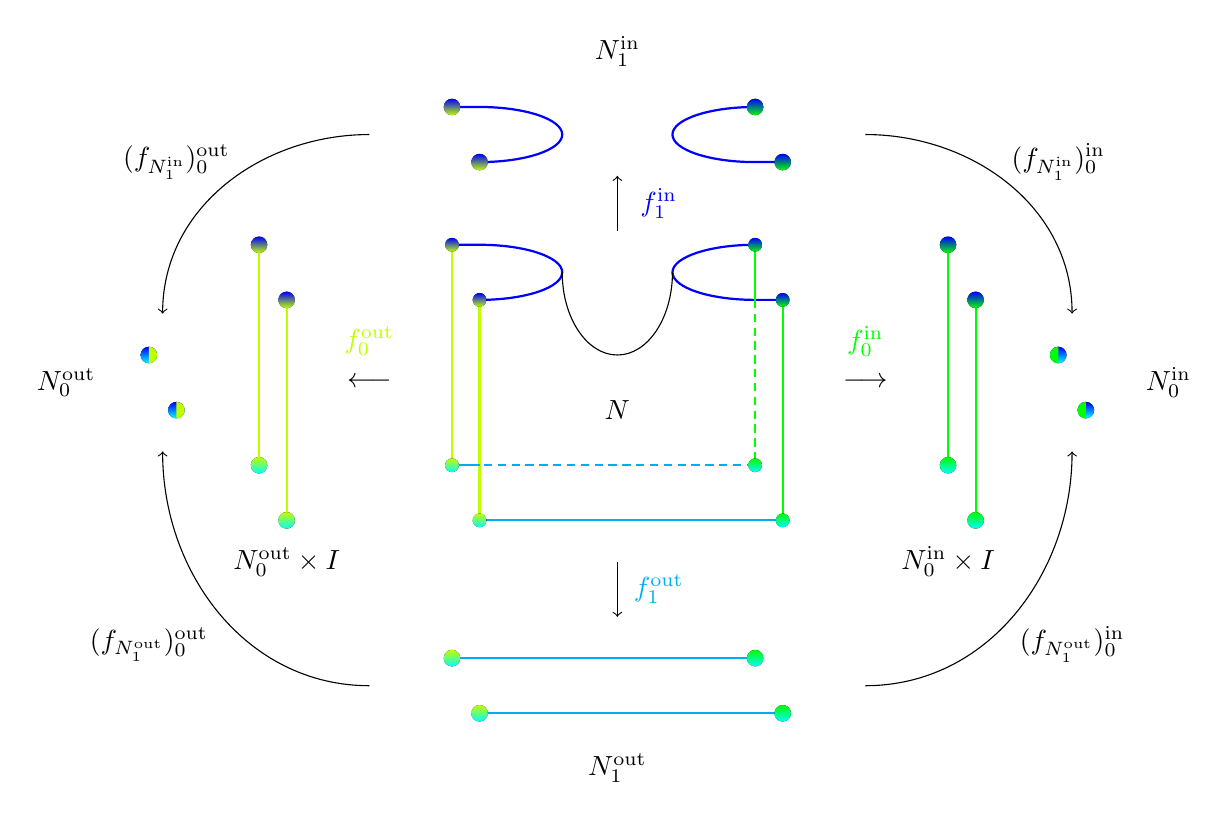
\begin{tikzpicture}[scale=3.5,thick]
  % top
  %edges
  \draw[blue] (1,3.5) arc (90:270:0.3cm and 0.1cm) -- (1.1,3.3);
  \draw[blue] (-0.1,3.5) -- (0,3.5) arc (90:-90:0.3cm and 0.1cm);
  %corners
  \fill[top color=blue,bottom color=green] (1,3.5) circle (0.3mm);
  \fill[top color=blue,bottom color=green] (1.1,3.3) circle (0.3mm);
  \fill[top color=blue,bottom color=lime] (-0.1,3.5) circle (0.3mm);
  \fill[top color=blue,bottom color=lime] (0,3.3) circle (0.3mm);
  %labels
  \node[at={(0.5,3.7)}]{$N_{1}^{\mathrm{in}}$};
  \draw[thin,->] (0.5,3.05) -- (0.5,3.25);
  \node[at={(0.65,3.15)},text=blue]{$f_{1}^{\mathrm{in}}$};
  
  % main
  %edges
  \draw[blue] (-0.1,3) -- (0,3) arc (90:-90:0.3cm and 0.1cm);
  \draw[blue] (1,3) arc (90:270:0.3cm and 0.1cm) -- (1.1,2.8);
  \draw[lime] (0,2.8) -- (0,2);
  \draw[lime] (-0.1,3) -- (-0.1,2.2);
  \draw[green] (1.1,2.8) -- (1.1,2);
  \draw[green] (1,3) -- (1,2.8);
  \draw[green,densely dashed] (1,2.8) -- (1,2.2);
  \draw[cyan,densely dashed] (1,2.2) -- (0,2.2);
  \draw[cyan] (1.1,2) -- (0,2);
  \draw[cyan] (-0.1,2.2) -- (0,2.2);
  \draw[thin] (0.3,2.9) arc (180:360:0.2cm and 0.3cm);
  %corners
  \fill[top color=blue,bottom color=green] (1,3) circle (0.25mm);
  \fill[top color=blue,bottom color=green] (1.1,2.8) circle (0.25mm);
  \fill[top color=blue,bottom color=lime] (-0.1,3) circle (0.25mm);
  \fill[top color=blue,bottom color=lime] (0,2.8) circle (0.25mm);
  \fill[top color=green,bottom color=cyan] (1,2.2) circle (0.25mm);
  \fill[top color=green,bottom color=cyan] (1.1,2) circle (0.25mm);
  \fill[top color=lime,bottom color=cyan] (-0.1,2.2) circle (0.25mm);
  \fill[top color=lime,bottom color=cyan] (0,2) circle (0.25mm);
  %labels
  \node[at={(0.5,2.4)}]{$N$};
  
  % bottom
  %edges
  \draw[cyan] (-0.1,1.5) -- (1,1.5) (0,1.3) -- (1.1,1.3);
  %corners
  \fill[top color=lime,bottom color=cyan] (-0.1,1.5) circle (0.3mm);
  \fill[top color=lime,bottom color=cyan] (0,1.3) circle (0.3mm);
  \fill[top color=green,bottom color=cyan] (1,1.5) circle (0.3mm);
  \fill[top color=green,bottom color=cyan] (1.1,1.3) circle (0.3mm);
  %labels
  \node[at={(0.5,1.1)}]{$N_{1}^{\mathrm{out}}$};
  \draw[thin,<-] (0.5,1.65) -- (0.5,1.85);
  \node[at={(0.65,1.75)},text=cyan]{$f_{1}^{\mathrm{out}}$};
  
  % left
  %edges
  \draw[lime] (-0.7,2.8) -- (-0.7,2) (-0.8,3) -- (-0.8,2.2);
  %corners
  \fill[top color=blue,bottom color=lime] (-0.7,2.8) circle (0.3mm);
  \fill[top color=blue,bottom color=lime] (-0.8,3) circle (0.3mm);
  \fill[top color=lime,bottom color=cyan] (-0.7,2) circle (0.3mm);
  \fill[top color=lime,bottom color=cyan] (-0.8,2.2) circle (0.3mm);
  \fill[top color=blue,bottom color=cyan] (-1.1,2.4) circle (0.3mm);
  \fill[lime] (-1.1,2.37) arc (270:450:0.3mm);
  \fill[top color=blue,bottom color=cyan] (-1.2,2.6) circle (0.3mm);
  \fill[lime] (-1.2,2.57) arc (270:450:0.3mm);
  %labels
  \node[at={(-1.5,2.5)}]{$N_{0}^{\mathrm{out}}$};
  \node[at={(-0.7,1.85)}]{$N_{0}^{\mathrm{out}} \times I$};
  \node[at={(-0.4,2.65)},text=lime]{$f_{0}^{\mathrm{out}}$};
  \node[at={(-0.4,2.5)}]{$\longleftarrow$};
  \draw[thin,<-] (-1.15,2.75) to [out=90,in=180] (-0.4,3.4);
  \draw[thin,<-] (-1.15,2.25) to [out=270,in=180] (-0.4,1.4);
  \node[at={(-1.1,3.3)}]{$(f_{N_{1}^{\mathrm{in}}})_{0}^{\mathrm{out}}$};
  \node[at={(-1.2,1.55)}]{$(f_{N_{1}^{\mathrm{out}}})_{0}^{\mathrm{out}}$};
  
  % right
  %edges
  \draw[green] (1.8,2.8) -- (1.8,2) (1.7,3) -- (1.7,2.2);
  %corners
  \fill[top color=blue,bottom color=green] (1.8,2.8) circle (0.3mm);
  \fill[top color=blue,bottom color=green] (1.7,3) circle (0.3mm);
  \fill[top color=green,bottom color=cyan] (1.8,2) circle (0.3mm);
  \fill[top color=green,bottom color=cyan] (1.7,2.2) circle (0.3mm);
  \fill[top color=blue,bottom color=cyan] (2.2,2.4) circle (0.3mm);
  \fill[green] (2.2,2.43) arc (90:270:0.3mm);
  \fill[top color=blue,bottom color=cyan] (2.1,2.6) circle (0.3mm);
  \fill[green] (2.1,2.63) arc (90:270:0.3mm);
  %labels
  \node[at={(2.5,2.5)}]{$N_{0}^{\mathrm{in}}$};
  \node[at={(1.7,1.85)}]{$N_{0}^{\mathrm{in}} \times I$};
  \node[at={(1.4,2.65)},text=green]{$f_{0}^{\mathrm{in}}$};
  \node[at={(1.4,2.5)}]{$\longrightarrow$};
  \draw[thin,<-] (2.15,2.75) to [out=90,in=0] (1.4,3.4);
  \draw[thin,<-] (2.15,2.25) to [out=270,in=0] (1.4,1.4);
  \node[at={(2.1,3.3)}]{$(f_{N_{1}^{\mathrm{in}}})_{0}^{\mathrm{in}}$};
  \node[at={(2.15,1.55)}]{$(f_{N_{1}^{\mathrm{out}}})_{0}^{\mathrm{in}}$};
\end{tikzpicture}
\caption{Illustration of the saddle}
\label{fig:saddle}
\end{figure}
\\
\end{exa}
\begin{prf}
Once again, the technical details can be filled in as an exercise.
\\
\phantom{proven}
\hfill
$\Box$
\end{prf}
Remember that given two ordinary $1$-cobordisms $M_{1},M_{2}$ such that the target of $M_{1}$ and the source of $M_{2}$ are the same, then the two can be glued together along the common boundary to yield a new $1$-cobordism with source the source of $M_{1}$ and target the target of $M_{2}$. Similarly, two $k$-cobordisms $M_{1},M_{2}$ can be glued together, but now there are $k$ directions in which one can glue. If the $i$-target of $M_{1}$ and the $i$-source of $M_{2}$ are the same - which implies that the corresponding $j$-boundaries for $j < i$ are the same for $M_{1}$ and $M_{2}$ - then the two $k$-cobordisms can be glued along this common part of the $i$-boundary to yield a new $k$-cobordism and this can be done for $0 \leq i \leq k-1$. The resulting $k$-cobordism has as $i$-source the $i$-source of $M_{1}$ and as $i$-target the $i$-target of $M_{2}$ and hence the same $j$-boundaries as $M_{1}$ and $M_{2}$ for $j < i$. For the other $j > i$ the $j$-source and $j$-target is the gluing of, respectively, the $j$-sources and $j$-targets of $M_{1}$ and $M_{2}$ along their respective common restriction of the $i$-boundary along which $M_{1}$ and $M_{2}$ are glued. This hopefully becomes clear in the following example.
\\
\begin{exa}
\label{exa:gluing}
As an example for gluing higher cobordisms consider the $2$-dimensional $2$-cobordism in figure \ref{fig:halfcyl}, denoted $M$.
\\
\begin{figure}[h!]
\centering
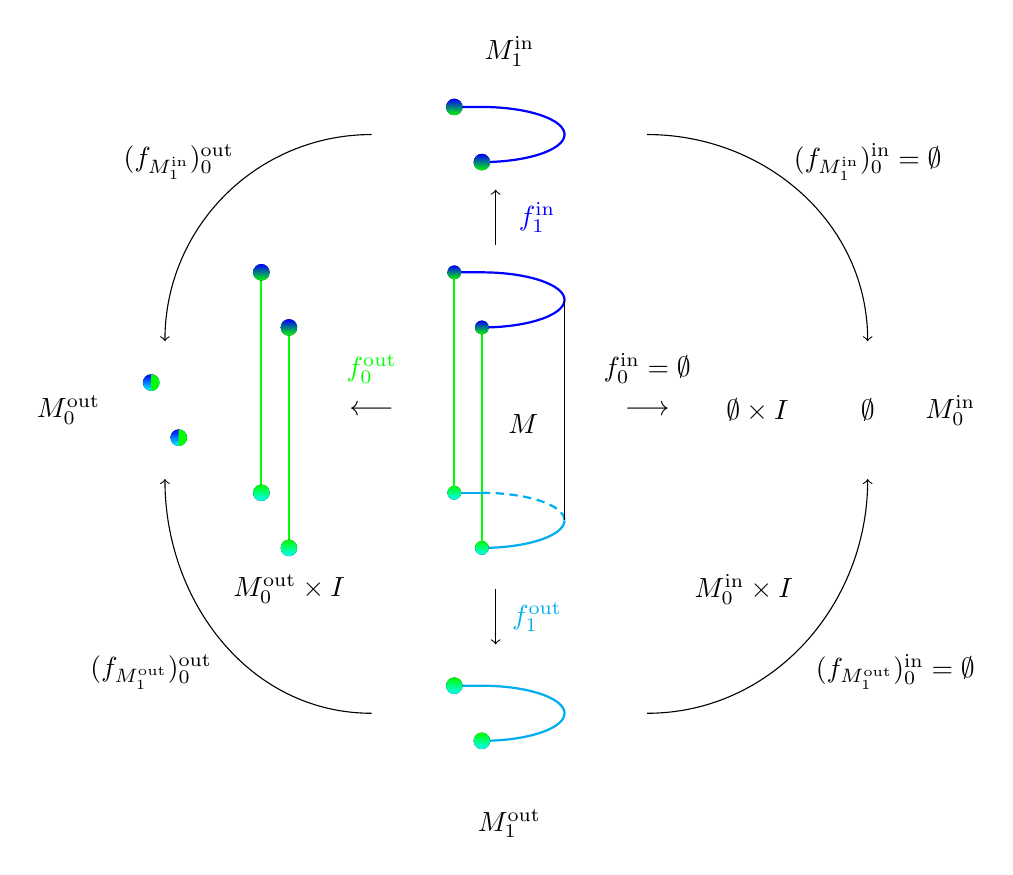
\begin{tikzpicture}[scale=3.5,thick]
  % top
  %edges
  \draw[blue] (-0.1,3.6) -- (0,3.6) arc (90:-90:0.3cm and 0.1cm);
  %corners
  \fill[top color=blue,bottom color=green] (-0.1,3.6) circle (0.3mm);
  \fill[top color=blue,bottom color=green] (0,3.4) circle (0.3mm);
  %labels
  \node[at={(0.1,3.8)}]{$M_{1}^{\mathrm{in}}$};
  \draw[thin,->] (0.05,3.1) -- (0.05,3.3);
  \node[at={(0.2,3.2)},text=blue]{$f_{1}^{\mathrm{in}}$};
  
  % main
  %edges
  \draw[blue] (-0.1,3) -- (0,3) arc (90:-90:0.3cm and 0.1cm);
  \draw[green] (0,2.8) -- (0,2);
  \draw[green] (-0.1,3) -- (-0.1,2.2);
  \draw[cyan] (-0.1,2.2) -- (0,2.2);
  \draw[cyan,densely dashed] (0,2.2) arc (90:0:0.3cm and 0.1cm);
  \draw[cyan] (0.3,2.1) arc (0:-90:0.3cm and 0.1cm);
  \draw[thin] (0.3,2.9) -- (0.3,2.1);
  %corners
  \fill[top color=blue,bottom color=green] (-0.1,3) circle (0.25mm);
  \fill[top color=blue,bottom color=green] (0,2.8) circle (0.25mm);
  \fill[top color=green,bottom color=cyan] (-0.1,2.2) circle (0.25mm);
  \fill[top color=green,bottom color=cyan] (0,2) circle (0.25mm);
  %labels
  \node[at={(0.15,2.45)}]{$M$};
  
  % bottom
  %edges
  \draw[cyan] (-0.1,1.5) -- (0,1.5) arc (90:-90:0.3cm and 0.1cm);
  %corners
  \fill[top color=green,bottom color=cyan] (-0.1,1.5) circle (0.3mm);
  \fill[top color=green,bottom color=cyan] (0,1.3) circle (0.3mm);
  %labels
  \node[at={(0.1,1)}]{$M_{1}^{\mathrm{out}}$};
  \draw[thin,<-] (0.05,1.65) -- (0.05,1.85);
  \node[at={(0.2,1.75)},text=cyan]{$f_{1}^{\mathrm{out}}$};
  
  % left
  %edges
  \draw[green] (-0.7,2.8) -- (-0.7,2) (-0.8,3) -- (-0.8,2.2);
  %corners
  \fill[top color=blue,bottom color=green] (-0.7,2.8) circle (0.3mm);
  \fill[top color=blue,bottom color=green] (-0.8,3) circle (0.3mm);
  \fill[top color=green,bottom color=cyan] (-0.7,2) circle (0.3mm);
  \fill[top color=green,bottom color=cyan] (-0.8,2.2) circle (0.3mm);
  \fill[top color=blue,bottom color=cyan] (-1.1,2.4) circle (0.3mm);
  \fill[green] (-1.1,2.37) arc (270:450:0.3mm);
  \fill[top color=blue,bottom color=cyan] (-1.2,2.6) circle (0.3mm);
  \fill[green] (-1.2,2.57) arc (270:450:0.3mm);
  %labels
  \node[at={(-1.5,2.5)}]{$M_{0}^{\mathrm{out}}$};
  \node[at={(-0.7,1.85)}]{$M_{0}^{\mathrm{out}} \times I$};
  \node[at={(-0.4,2.65)},text=green]{$f_{0}^{\mathrm{out}}$};
  \node[at={(-0.4,2.5)}]{$\longleftarrow$};
  \draw[thin,<-] (-1.15,2.75) to [out=90,in=180] (-0.4,3.5);
  \draw[thin,<-] (-1.15,2.25) to [out=270,in=180] (-0.4,1.4);
  \node[at={(-1.1,3.4)}]{$(f_{M_{1}^{\mathrm{in}}})_{0}^{\mathrm{out}}$};
  \node[at={(-1.2,1.55)}]{$(f_{M_{1}^{\mathrm{out}}})_{0}^{\mathrm{out}}$};
  
  % right
  %edges
  \node[at={(1,2.5)}]{$\emptyset \times I$};
  %corners
  \node[at={(1.4,2.5)}]{$\emptyset$};
  %labels
  \node[at={(1.7,2.5)}]{$M_{0}^{\mathrm{in}}$};
  \node[at={(0.95,1.85)}]{$M_{0}^{\mathrm{in}} \times I$};
  \node[at={(0.6,2.65)}]{$f_{0}^{\mathrm{in}} = \emptyset$};
  \node[at={(0.6,2.5)}]{$\longrightarrow$};
  \draw[thin,<-] (1.4,2.75) to [out=90,in=0] (0.6,3.5);
  \draw[thin,<-] (1.4,2.25) to [out=270,in=0] (0.6,1.4);
  \node[at={(1.4,3.4)}]{$(f_{M_{1}^{\mathrm{in}}})_{0}^{\mathrm{in}} = \emptyset$};
  \node[at={(1.5,1.55)}]{$(f_{M_{1}^{\mathrm{out}}})_{0}^{\mathrm{in}} = \emptyset$};
\end{tikzpicture}
\caption{$2$-cobordism whose $0$-target is the same as the $0$-source of the saddle}
\label{fig:halfcyl}
\end{figure}
\clearpage
Gluing this to the saddle $N$ from example \ref{exa:saddle} along $N_{0}^{\mathrm{in}} = M_{0}^{\mathrm{out}}$ results in the $2$-dimensional $2$-cobordism depicted in figure \ref{fig:glued}.
\\
\begin{figure}[h!]
\centering
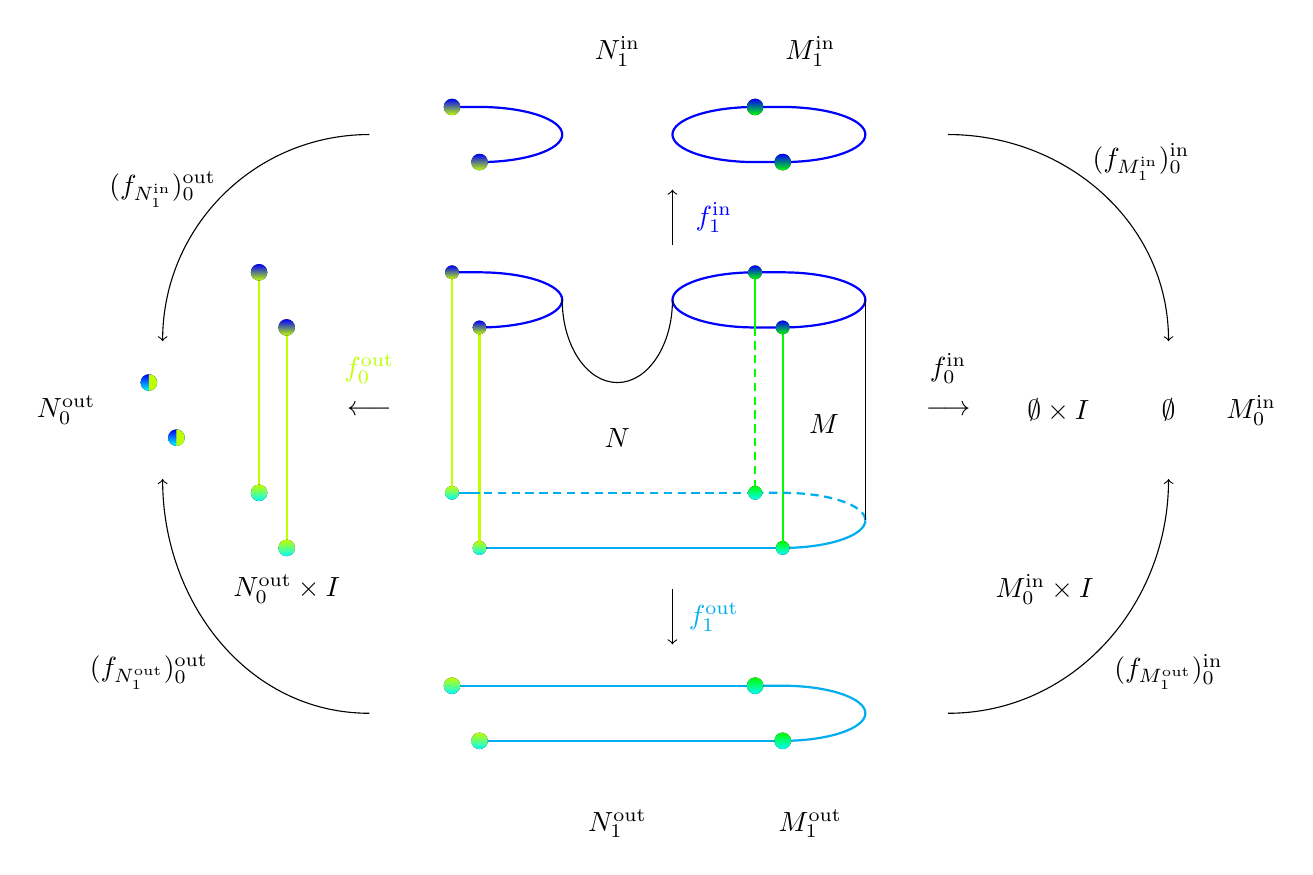
\begin{tikzpicture}[scale=3.5,thick]
  % top
  %edges
  \draw[blue] (1,3.6) arc (90:270:0.3cm and 0.1cm) -- (1.1,3.4);
  \draw[blue] (1,3.6) -- (1.1,3.6) arc (90:-90:0.3cm and 0.1cm);
  \draw[blue] (-0.1,3.6) -- (0,3.6) arc (90:-90:0.3cm and 0.1cm);
  %corners
  \fill[top color=blue,bottom color=green] (1,3.6) circle (0.3mm);
  \fill[top color=blue,bottom color=green] (1.1,3.4) circle (0.3mm);
  \fill[top color=blue,bottom color=lime] (-0.1,3.6) circle (0.3mm);
  \fill[top color=blue,bottom color=lime] (0,3.4) circle (0.3mm);
  %labels
  \node[at={(0.5,3.8)}]{$N_{1}^{\mathrm{in}}$};
  \node[at={(1.2,3.8)}]{$M_{1}^{\mathrm{in}}$};
  \draw[thin,->] (0.7,3.1) -- (0.7,3.3);
  \node[at={(0.85,3.2)},text=blue]{$f_{1}^{\mathrm{in}}$};
  
  % main
  %edges
  \draw[blue] (-0.1,3) -- (0,3) arc (90:-90:0.3cm and 0.1cm);
  \draw[blue] (1,3) arc (90:270:0.3cm and 0.1cm) -- (1.1,2.8);
  \draw[blue] (1,3) -- (1.1,3) arc (90:-90:0.3cm and 0.1cm);
  \draw[lime] (0,2.8) -- (0,2);
  \draw[lime] (-0.1,3) -- (-0.1,2.2);
  \draw[green] (1.1,2.8) -- (1.1,2);
  \draw[green] (1,3) -- (1,2.8);
  \draw[green,densely dashed] (1,2.8) -- (1,2.2);
  \draw[cyan,densely dashed] (1,2.2) -- (0,2.2);
  \draw[cyan] (1.1,2) -- (0,2);
  \draw[cyan] (-0.1,2.2) -- (0,2.2);
  \draw[cyan,densely dashed] (1,2.2) -- (1.1,2.2) arc (90:0:0.3cm and 0.1cm);
  \draw[cyan] (1.4,2.1) arc (0:-90:0.3cm and 0.1cm);
  \draw[thin] (0.3,2.9) arc (180:360:0.2cm and 0.3cm);
  \draw[thin] (1.4,2.9) -- (1.4,2.1);
  %corners
  \fill[top color=blue,bottom color=green] (1,3) circle (0.25mm);
  \fill[top color=blue,bottom color=green] (1.1,2.8) circle (0.25mm);
  \fill[top color=blue,bottom color=lime] (-0.1,3) circle (0.25mm);
  \fill[top color=blue,bottom color=lime] (0,2.8) circle (0.25mm);
  \fill[top color=green,bottom color=cyan] (1,2.2) circle (0.25mm);
  \fill[top color=green,bottom color=cyan] (1.1,2) circle (0.25mm);
  \fill[top color=lime,bottom color=cyan] (-0.1,2.2) circle (0.25mm);
  \fill[top color=lime,bottom color=cyan] (0,2) circle (0.25mm);
  %labels
  \node[at={(0.5,2.4)}]{$N$};
  \node[at={(1.25,2.45)}]{$M$};
  
  % bottom
  %edges
  \draw[cyan] (-0.1,1.5) -- (1,1.5) (0,1.3) -- (1.1,1.3);
  \draw[cyan] (1,1.5) -- (1.1,1.5) arc (90:-90:0.3cm and 0.1cm);
  %corners
  \fill[top color=lime,bottom color=cyan] (-0.1,1.5) circle (0.3mm);
  \fill[top color=lime,bottom color=cyan] (0,1.3) circle (0.3mm);
  \fill[top color=green,bottom color=cyan] (1,1.5) circle (0.3mm);
  \fill[top color=green,bottom color=cyan] (1.1,1.3) circle (0.3mm);
  %labels
  \node[at={(0.5,1)}]{$N_{1}^{\mathrm{out}}$};
  \node[at={(1.2,1)}]{$M_{1}^{\mathrm{out}}$};
  \draw[thin,<-] (0.7,1.65) -- (0.7,1.85);
  \node[at={(0.85,1.75)},text=cyan]{$f_{1}^{\mathrm{out}}$};
  
  % left
  %edges
  \draw[lime] (-0.7,2.8) -- (-0.7,2) (-0.8,3) -- (-0.8,2.2);
  %corners
  \fill[top color=blue,bottom color=lime] (-0.7,2.8) circle (0.3mm);
  \fill[top color=blue,bottom color=lime] (-0.8,3) circle (0.3mm);
  \fill[top color=lime,bottom color=cyan] (-0.7,2) circle (0.3mm);
  \fill[top color=lime,bottom color=cyan] (-0.8,2.2) circle (0.3mm);
  \fill[top color=blue,bottom color=cyan] (-1.1,2.4) circle (0.3mm);
  \fill[lime] (-1.1,2.37) arc (270:450:0.3mm);
  \fill[top color=blue,bottom color=cyan] (-1.2,2.6) circle (0.3mm);
  \fill[lime] (-1.2,2.57) arc (270:450:0.3mm);
  %labels
  \node[at={(-1.5,2.5)}]{$N_{0}^{\mathrm{out}}$};
  \node[at={(-0.7,1.85)}]{$N_{0}^{\mathrm{out}} \times I$};
  \node[at={(-0.4,2.65)},text=lime]{$f_{0}^{\mathrm{out}}$};
  \node[at={(-0.4,2.5)}]{$\longleftarrow$};
  \draw[thin,<-] (-1.15,2.75) to [out=90,in=180] (-0.4,3.5);
  \draw[thin,<-] (-1.15,2.25) to [out=270,in=180] (-0.4,1.4);
  \node[at={(-1.15,3.3)}]{$(f_{N_{1}^{\mathrm{in}}})_{0}^{\mathrm{out}}$};
  \node[at={(-1.2,1.55)}]{$(f_{N_{1}^{\mathrm{out}}})_{0}^{\mathrm{out}}$};
  
  % right
  %edges
  \node[at={(2.1,2.5)}]{$\emptyset \times I$};
  %corners
  \node[at={(2.5,2.5)}]{$\emptyset$};
  %labels
  \node[at={(2.8,2.5)}]{$M_{0}^{\mathrm{in}}$};
  \node[at={(2.05,1.85)}]{$M_{0}^{\mathrm{in}} \times I$};
  \node[at={(1.7,2.65)}]{$f_{0}^{\mathrm{in}}$};
  \node[at={(1.7,2.5)}]{$\longrightarrow$};
  \draw[thin,<-] (2.5,2.75) to [out=90,in=0] (1.7,3.5);
  \draw[thin,<-] (2.5,2.25) to [out=270,in=0] (1.7,1.4);
  \node[at={(2.4,3.4)}]{$(f_{M_{1}^{\mathrm{in}}})_{0}^{\mathrm{in}}$};
  \node[at={(2.5,1.55)}]{$(f_{M_{1}^{\mathrm{out}}})_{0}^{\mathrm{in}}$};
\end{tikzpicture}
\caption{$2$-cobordism obtained by gluing the one from figure \ref{fig:halfcyl} and the saddle}
\label{fig:glued}
\end{figure}
\\
\end{exa}
\begin{prf}
Filling in the technical details can be done as an exercise.
\\
\phantom{proven}
\hfill
$\Box$
\end{prf}
There are several subtleties involved in this process of gluing, some of which are similar to the case of ordinary cobordisms, for example, the gluings of $k$-cobordisms are achieved by choosing appropriate collars, which is always possible. Therefore the resulting $k$-cobordisms obtained by gluing are well-defined only up to equivalence of $k$-cobordisms. We will not press the details further here and refer the interested reader to \cite{d37d0fca} instead where the $2$-dimensional case is treated extensively and illustrates all the details.
